%%%%%%%%%%%%%%%%%%%%%%%%%%%%%%%%%%%%%%%%%%%%%%%%%%%%%%%%%%%%%%%%%%%%%%%%%%%%%%%%
% Limit_Intepretation.tex: Select of showering and tracking events:
%%%%%%%%%%%%%%%%%%%%%%%%%%%%%%%%%%%%%%%%%%%%%%%%%%%%%%%%%%%%%%%%%%%%%%%%%%%%%%%%
\chapter{Limit Interpretation}
\label{Limit_Results_and_Intepretation_Chapter}
%%%%%%%%%%%%%%%%%%%%%%%%%%%%%%%%%%%%%%%%%%%%%%%%%%%%%%%%%%%%%%%%%%%%%%%%%%%%%%%%

Using the $CL_{s}$ technique, the HiggsCombine tool produces an upper limit along with the expected limit at different quantiles as the signal strength computed which is a ratio of Number of Signal events over the Number of Expected signal events i.e
\begin{equation}
 r = \frac {N^{Obs}}{N_{expect}}
\end{equation}
and using the equation as given in chapter 3 on the cross-section $\sigma = \frac{N}{\varepsilon\cdot A \cdot \mathscr{L}}$ and hence the observed cross-section upper limit is given as:

\begin{equation}
\sigma^{Obs}_{UL} = \frac{r\cdot N^{expect}}{\varepsilon\cdot A\cdot \mathscr{L}}
\end{equation}

where $\mathscr{L}$ is the integrated luminosity~(19\fbinv) and $\varepsilon$ and $A$ are the signal selection efficiency and Acceptance respectively.
In addition to the observed limits~(Solid black line), the uncertainties on the expected limits at 68\%/16\%~($\pm 1\sigma$) and at 98\%/2.5\%~($\pm 2\sigma$) provide the \colorbox{green}{GREEN} and \colorbox{yellow}{YELLOW} respectively, the error from the median~(50\%) expected limits~(dashed red line) shown in figure \ref{fig:SPS8_Ctau_Ulimit}.


%%%%%%%%%%%%%%%%%%%%%%%%%%%%%%%%%%%%%%%%%%%%%%%%%%%%%%%%%%%%%%%%%
\section{Signal Efficiency and Acceptance}
%%%%%%%%%%%%%%%%%%%%%%%%%%%%%%%%%%%%%%%%%%%%%%%%%%%%%%%%%%%%%%%%%
The efficiency times acceptance~($\varepsilon \times A$) combined as one is seen the figure \ref{fig:EffAcc}.
\begin{center}
%\includegraphics[width=0.49\textwidth,height=0.5\textwidth]
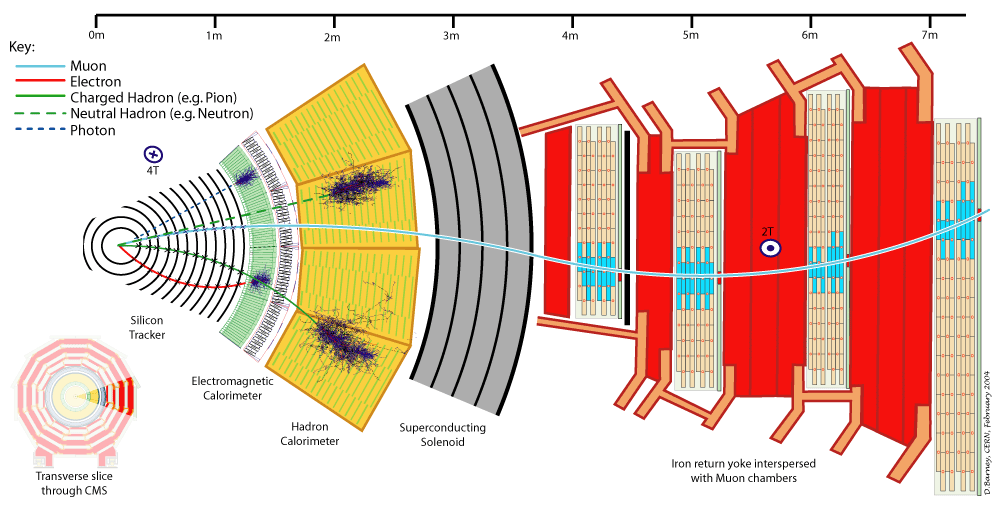
\includegraphics[scale=0.2]{THESISPLOTS/CMS_Slice.png}
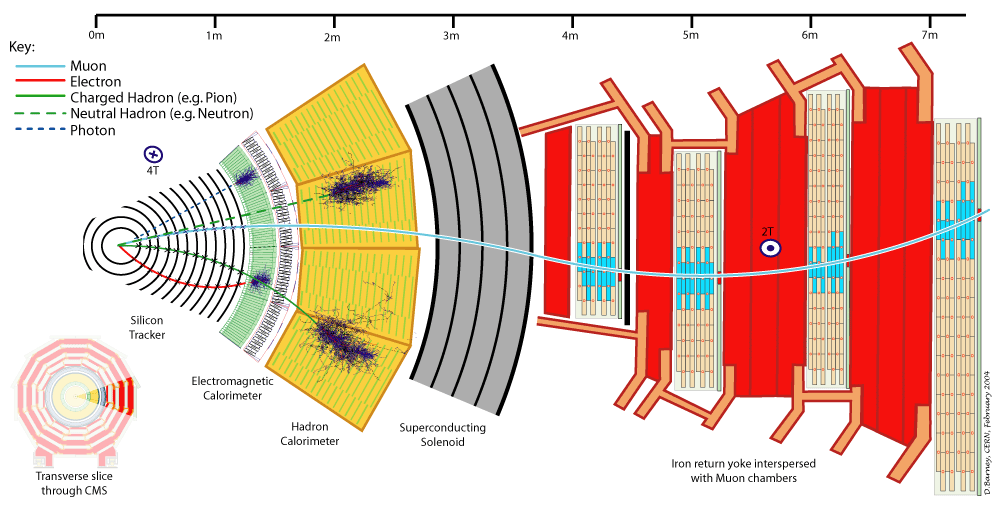
\includegraphics[scale=0.2]{THESISPLOTS/CMS_Slice.png}
\captionof{figure}{Signal efficiency $\times$ Acceptance for signal events passing our events selection for the SPS8(left) and GGM(right) models. The acceptance are photons with $t > 3$~ns.}
\label{fig:EffAcc}
\end{center}


\par
The $\frac{N^{expet}}{\mathscr{L}}$ defines the expected signal cross section which is obtained from a given signal model. In our scenario, our choice of signal model we  want to produce exclusion limits on the possible production and decay of a long-lived particle described by this signal model is GMSB.
Thus the interpretation of our search analysis is given within the context of any GMSB model with a long-live neutral particle decaying to a photon and gravitino. Such a model is the minimal GMSB or the SPS8 model and the general GMSB model. However, the results provided are based on interpretation within the context of the SPS8 model.
In GMSB, the neutralino $\tilde{\chi^{0}_{1}}$ is the NLSP and decays to the gravitino $\tilde{G}$ the LSP~(as a result of R-parity conservation) in association with a very energetic photon $\gamma$. Because of the smallness in mass difference between the  $\tilde{\chi^{0}_{1}}$ and the $\tilde{G}$ as well as the coupling, the $\tilde{\chi^{0}_{1}}$ decay to $\tilde{G}$ is delayed and as a result, the photon emitted can arrive late in the calorimeter crystals.  Measuring the arrival time of the photon on ECAL crystals, we can extract important parameters of  theory of GMSB.




\begin{center}
\centering
\mbox{
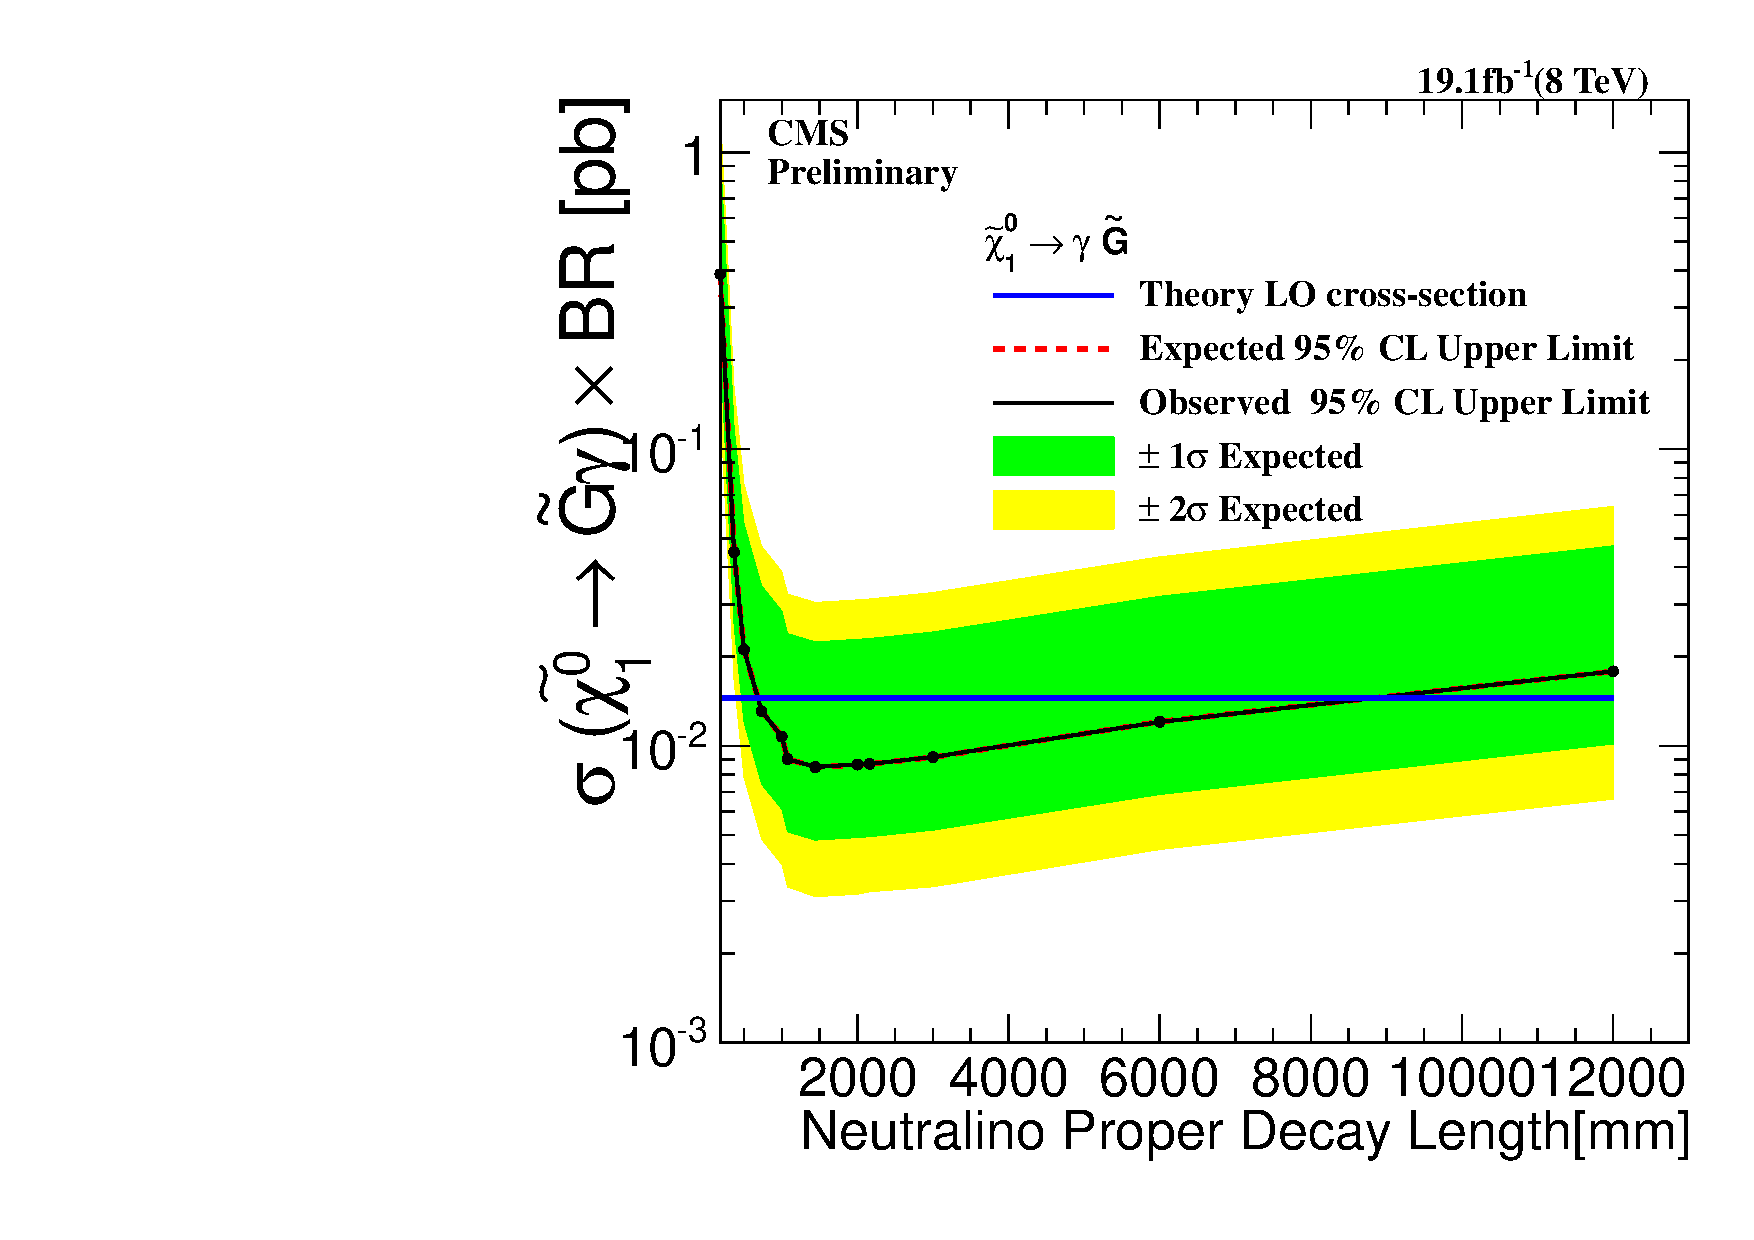
\includegraphics[width=5in]{THESISPLOTS/Neutralino_CrossSecTimesBR_Uplimit.pdf}}
\captionof{figure}{Neutralino production cross section against proper delay length upper limit interpretation in SPS8 model.}
\label{fig:SPS8_Ctau_Ulimit}
\end{center}


In the SPS8 model, the parameter space for long-live neutralinos is govern by $\Lambda_{m}-c\tau$ 2-dimensional parameter space. For each $\Lambda_{m}$ point, we have a fixed neutralino mass with different proper lifetimes $c\tau$. We have obtained limits for $\Lambda_{m}$ ranging from $100$~TeV to $180$~TeV corresponding to lightest neutralino mass $m_{\tilde{\chi}^{0}_{1}}$ between $90$ to $255$~$GeV/c^{2}$ and proper lifetime $c\tau$ ranging from $250$ to $12000$~mm corresponding to $\tau_{\tilde{\chi}^{0}_{1}}$ from $0.8$~ns to $40$~ns.

For a given value of $\Lambda_{m} = 180$~TeV, we have a lightest neutralino production cross section times branching ratio plot shown in figure \ref{fig:SPS8_Ctau_Ulimit}, showing that the ECAL detector is sensitive to lightest neutralinos of mass $m_{\tilde{\chi}^{0}_{1}} = 255$~$GeV/c^{2}$ and life time upto $30$~ns and we are 95\% confident that we have not missed any neutralino whose mass is $m_{\tilde{\chi}^{0}_{1}} = 255$~$GeV/c^{2}$ and lifetime is $\tau \leq 30$~ns.
\mbox{}\\
For a given lifetime of $\tau = 20$~ns, we can also obtain upper limits on the production cross section times branching ratio when compared against their theoretically expected values for a lightest neutralino with mass ranging from $m_{\tilde{\chi}^{0}_{1}} = 90$~$GeV/c^{2}$ to $m_{\tilde{\chi}^{0}_{1}} = 255$~$GeV/c^{2}$. The observed upper limit on this cross section is $\sigma^{UP}_{\tilde{\chi}^{0}_{1}} \geq XX$~pb with proper lifetime of $\tau = 30$~ns.

\mbox{}\\
Using both the mass and proper lifetime of the lightest neutralino, we present possible 2-dimensional limits simulateneously on $m_{\tilde{\chi}^{0}_{1}}$ or $\Lambda_{m}$ and $c\tau$ or $\tau$ in the SPS8 model, comparing this with the result of previous experiments. This is shown in figure \ref{fig:limits}.

%\begin{figure}[!htb]
\begin{center}
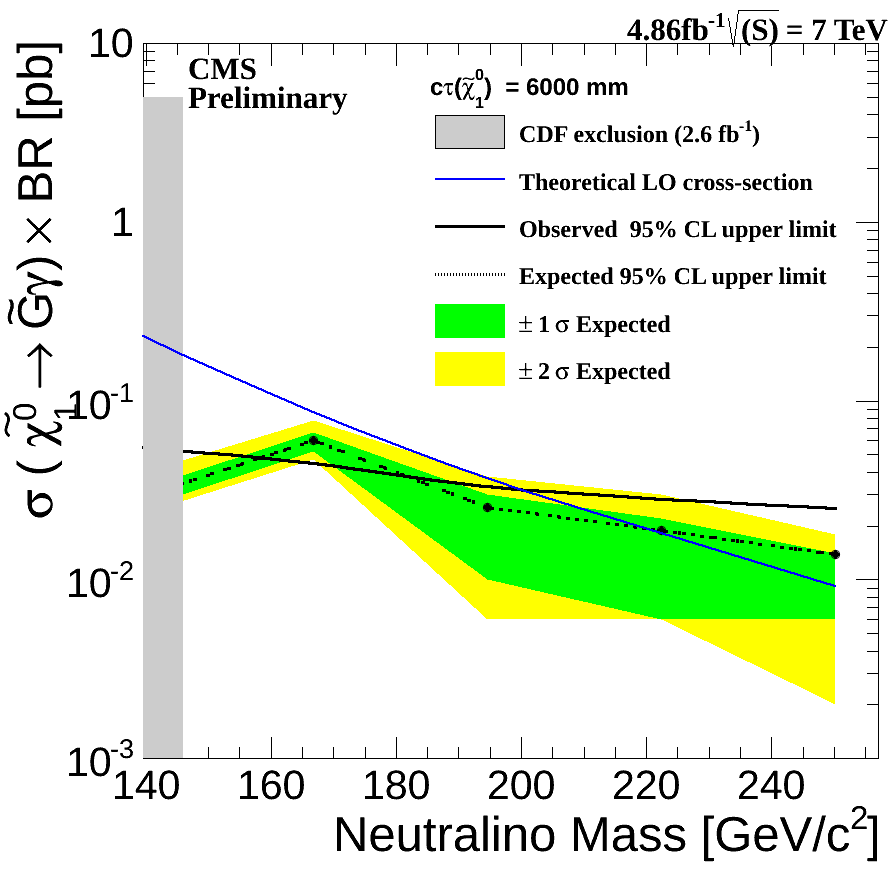
\includegraphics[width=0.49\textwidth,height=0.5\textwidth]{THESISPLOTS/Neutralino_XsecVsMAss_Exclusion_limit_6000.png}
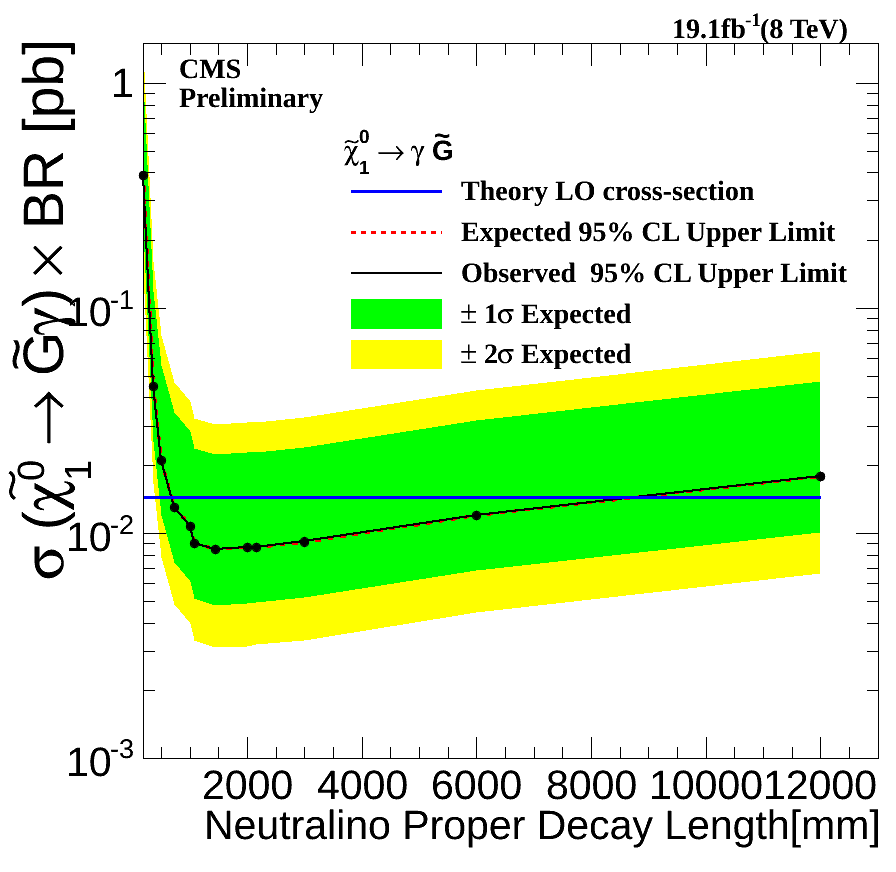
\includegraphics[width=0.49\textwidth,height=0.5\textwidth]{THESISPLOTS/Neutralino_CrossSecTimesBR_Uplimit.png}
\captionof{figure}{Neutralino production cross section against proper delay length upper limit at 95\% confidence levels interpretation in SPS8 model.}
\label{fig:limits}
\end{center}
%\end{figure}


\begin{center}
\centering
\mbox{
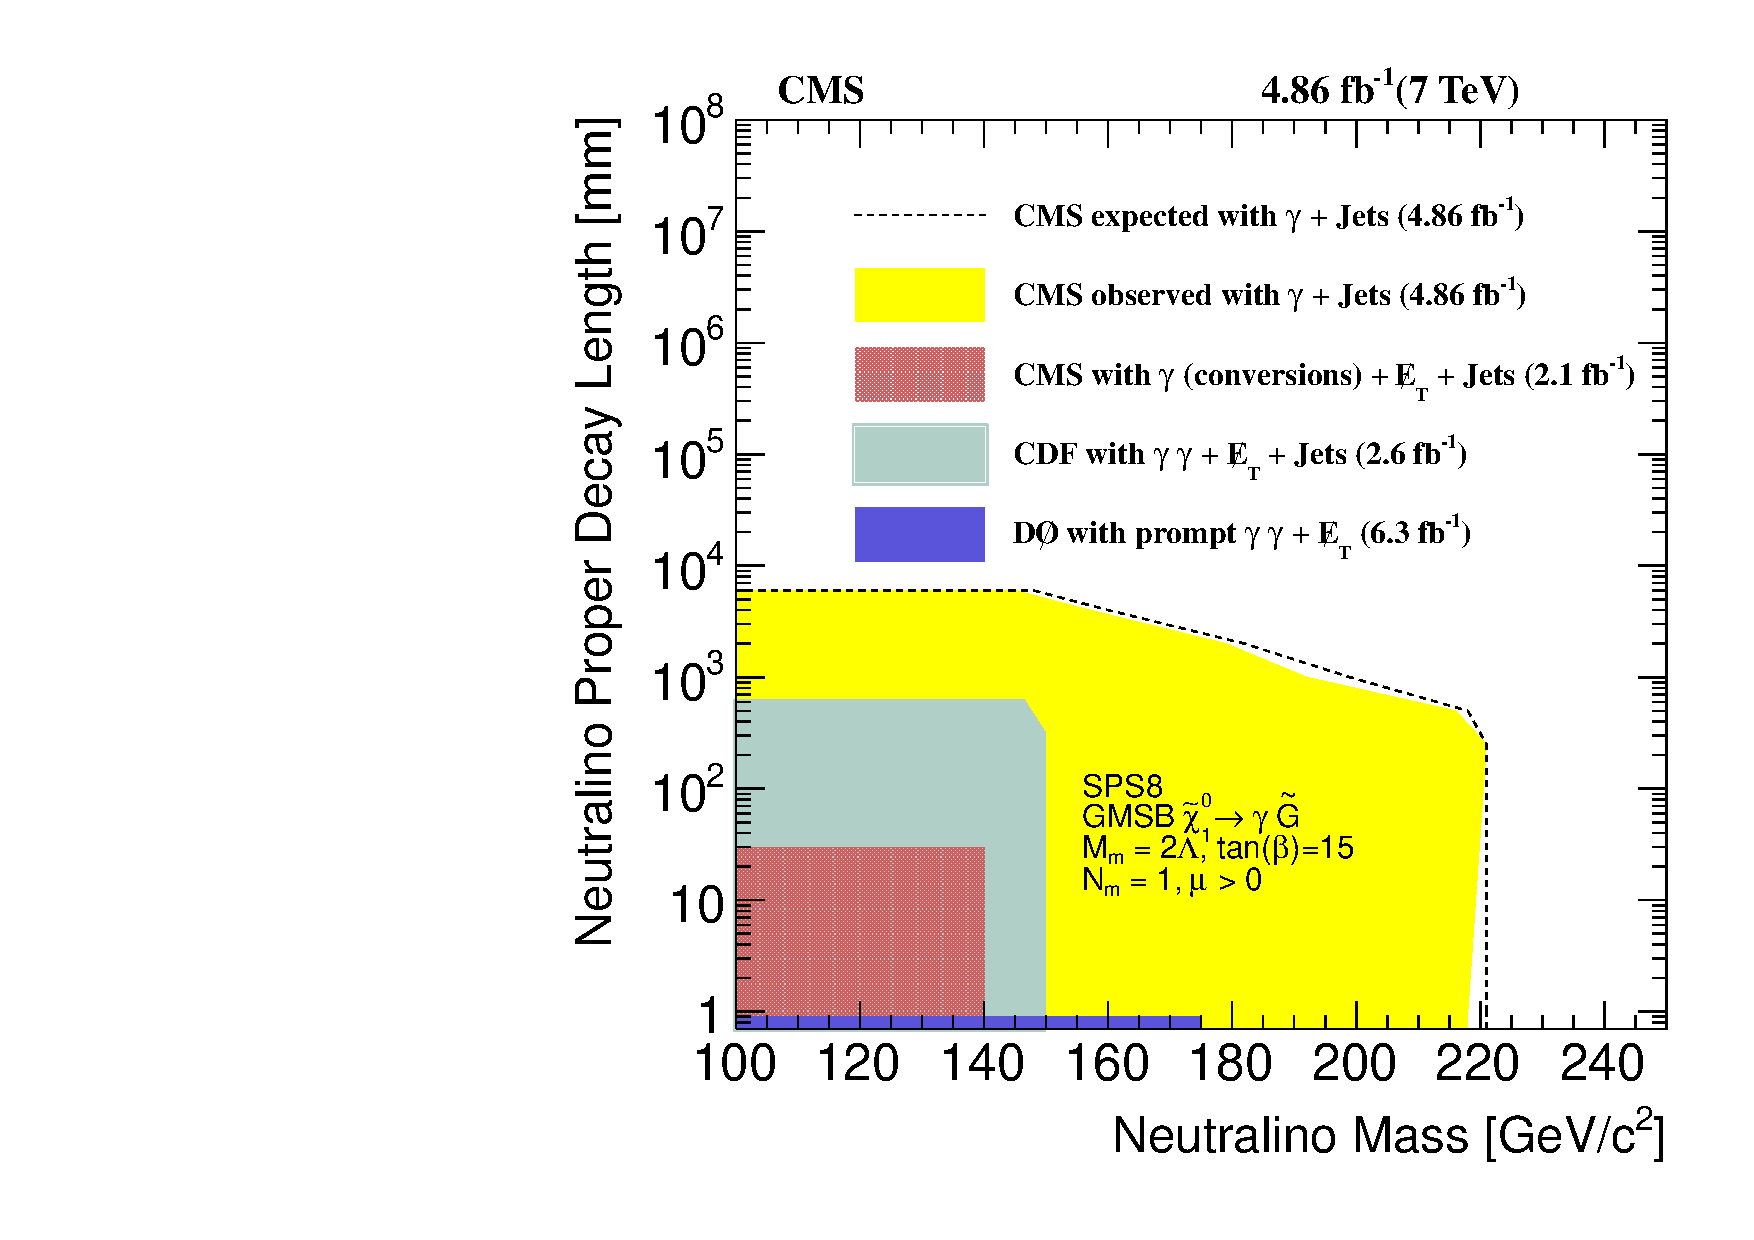
\includegraphics[width=5in]{THESISPLOTS/Neutralino_2D_exclusion.pdf} }
\captionof{figure}{Neutralino two dimensional exclusion limit of neutralino mass ($\Lambda$) against proper delay length upper limit interpretation in SPS8 model in the decay $\tilde{\chi}^{0}_{1} \rightarrow \gamma + \tilde{G}$ with limits from previous experiments shown.}
\label{fig:SPS8_Ulimit}
\end{center}


%%%%%%%%%%%%%%%%%%%%%%%%%%%%%%%%%%%%%%%%%%%%%%%%%%%%%%%%%%%%%%%%%%%%%%%%%%%%%%%%
%%%%%%%%%%%%%%%%%%%%%%%%%%%%%%%%%%%%%%%%%%%%%%%%%%%%%%%
%%%%%%%%%%%%%%%%%%%%%%%%%%%%%%%%%%%%%%%%%%%%%%%%%%%%%%%%%%%%%%%%%%%%%%%%%%%%%%%%
% Possible Future Analysis work!
%%%%%%%%%%%%%%%%%%%%%%%%%%%%%%%%%%%%%%%%%%%%%%%%%%%%%%%%%%%%%%%%%%%%%%%%%%%%%%%%
\section{Future Improvements}
%%%%%%%%%%%%%%%%%%%%%%%%%%%%%%%%%%%%%%%%%%%%%%%%%%%%%%%%%%%%%%%%%%%%

%%%%%%%%%%%%%%%%%%%%%%%%

\subsection{Beam Halo Monitoring Detector}
%\label{Beam Halo Procedure}
%%%%%%%%%%%%%%%%%%%%%%%%%%%%%%%%%%%%%%%%%%%%%%%%%%%%%%%%%%%%%%%%%%%%%%%%%%%%%%%%


%%%%%%%%%%%%%%%%%%%%%%%%%%%%%%%%%%%%%%%%%%%%%%%%%%%%%%%%%%%%%%%%%%%%%%%%%%%%%%%%
\subsection{Back-end Electronics upgrade HCAL}
%\label{hcal)back_end_Electronics}

%%%%%%%%%%%%%%%%%%%%%%%%%%%%%%%%%%%%%%%%%%%%%%%%%%%%%%%%%%%%%%%%%%%%%%%%%%%%%}}}
